\documentclass{article}

%% Preemptively pass options to avoid import conflicts.
\PassOptionsToPackage{linesnumbered,ruled,vlined}{algorithm2e}
\PassOptionsToPackage{capitalise,noabbrev}{cleveref}
\PassOptionsToPackage{margin=1in}{geometry}
\PassOptionsToPackage{pagebackref=true}{hyperref}
\PassOptionsToPackage{numbers,compress}{natbib}

\usepackage[abbrvbib,nohyperref,preprint]{jmlr2e}
\usepackage[ref]{leaf}
\usepackage{algorithm}
\usepackage{algpseudocode}

%% Cleveref settings
\crefname{equation}{}{}
\Crefname{equation}{}{}

% Heading arguments are {volume}{year}{pages}{date submitted}{date published}{paper id}{author-full-names}
%% \jmlrheading{}{}{}{}{}{}{}

% Short headings should be running head and authors last names
% \ShortHeadings{}{}

\firstpageno{1}

\begin{document}

\title{Collaborative Filtering using implicit feedback in the Million Song Dataset}

\author{%
\name Zheyuan Hu \email zh2095@nyu.edu \AND
\name Ye Eun Jeong \email yej208@nyu.edu \AND
\name Sanyam Kapoor \email sk6876@nyu.edu \AND
\name Hongmiao Yu \email hy1709@nyu.edu
}

% \author{}
% \editor{}

\maketitle

%\begin{abstract}%   <- trailing '%' for backward compatibility of .sty file
%
%\end{abstract}

\vspace{-2em}

\section{Introduction}

Recommender systems are the cornerstone of modern (internet) economy, with 
examples including furniture recommendation 
\citep{10.1145/3383313.3411550}, online dating 
\citep{10.1145/3383313.3411558}, video recommendations 
\citep{10.1145/3383313.3411555}, and user interface personalization 
\citep{10.1145/3383313.3411549}. Such systems seek to predict the 
\emph{rating}, or a \emph{preference} between a \emph{user} and an 
\emph{item}, and are traditionally classified into two types - 
\emph{Content-based} recommendations rely on a user's past behavior, 
whereas \emph{Collaborative filtering-based} recommendations rely on the 
idea of similarity between users \citep{Pazzani2004AFF}. In this report, we 
focus on the latter.

Collaborative filtering, first introduced by \citet{Goldberg1992UsingCF}, 
analyzes the relationship between users and interdependent items, to 
identify new user-item recommendations. The only required information is 
the user's past (potentially sparse) interaction with items. In that sense, 
the method is domain-free, and widely applicable. The Netflix Prize 
\citep{Bennett07thenetflix} demonstrated the superiority of matrix 
factorization based recommender systems \citep{koren2009}, and will be the 
basis of our method too.

The rest of the report is organized as follows: \cref{sec:methodology} 
summarizes the problem setup and methodology. \cref{sec:extensions} 
describes two extensions that we investigate. Finally, \cref{sec:results} 
presents the results for all our experiments.

\section{Methodology}\label{sec:methodology}

As alluded to earlier, we rely on matrix factorization approaches to 
collaborative filtering. In particular, latent factor models take a more 
holistic approach that use latent factors to explain the observed 
interactions, i.e. ratings or preferences. We follow the presentation in 
\citet{yifan2008}.

In general, each user $u \in \mathcal{U}$ is associated to a latent 
user-factor factor denoted by $x_u \in \reals^f$, and each item 
$i \in \mathcal{I}$ is associated to a latent item-factor denoted by 
$y_i \in \reals^f$. The prediction of the preference is given by the inner
product between each user-item factor pair $\widehat{r}_{ui} = x_u^Ty_i$.

This prediction is then compared to every observed interaction $r_{ui}$. 
We denote the set of all observed interactions, also known as the 
\emph{utility matrix} as $\mathcal{R}$. The learning objective is then 
given by the regularized squared loss error,
\begin{align}
\argmax \sum_{r_{ui} \in \mathcal{R}} \left( r_{ui} - x_u^T y_i \right)^2 + \lambda \left( \norm{x_u}^2 + \norm{y_i}^2 \right) \label{eq:rec_obj}
\end{align}

The maximization in \cref{eq:rec_obj} is over all the latent factor vectors 
$x_u$ and $y_i$ for all $u \in \mathcal{U}$, and for all 
$i \in \mathcal{I}$. The regularization parameter $\lambda$ allows us to 
avoid overfitting on the training dataset by avoiding overly complex latent
factors.

The objective presented in \cref{eq:rec_obj} relies on 
\emph{explicit feedback} in the data. Such data is often high quality, and 
is collected by explicit inputs from the users, for instance star ratings. 
Unfortunately, explicit feedback is costly, and often not available. In 
such cases, we rely on collecting indirect preference signals like clicks, 
play counts in music, viewing times, and so on. This data is known as 
\emph{implicit feedback}, and is much cheaper to collect.

In this report, we focus on datasets with implicit feedback. As described 
earlier, we only have proxy measures of preference. First, we model each 
interaction as a binary variable $p_{ui}$, which is one for every positive
interaction, defined using the indicator function $\mathbb{I}$ as $p_{ui} = \mathbb{I}\left[ r_{ui} > 0 \right]$.

We can still rely on the general objective formulated in \cref{eq:rec_obj},
but now need to adjust the definition of $r_{ui}$ to faithfully represent 
some notion of \emph{confidence}. The assumption is that a higher value of 
$r_{ui}$ represents a stronger preference, and therefore a violation in the 
objective should be penalized more. Therefore, we introduce a weighting 
term $c_{ui} = 1 + \alpha r_{ui}$, where $\alpha$ is a scaling parameter to indicate stronger preference for 
higher $r_{ui}$ values. The new objective for implicit datasets in can then 
be written as a weighted version of \cref{eq:rec_obj} as,
\begin{align}
\argmax \left[ \sum_{r_{ui} \in \mathcal{R}} c_{ui}\left( p_{ui} - x_u^T y_i \right)^2 \right] + \lambda \left( \sum_{u \in \mathcal{U}} \norm{x_u}^2 + \sum_{i \in \mathcal{I}} \norm{y_i}^2 \right) \label{eq:rec_obj_implicit}	
\end{align}

As proposed by \citep{koren2009}, alternating least squares (ALS) algorithm 
is used to optimize \cref{eq:rec_obj_implicit}. This allows the objective 
to be convex, and easier to optimize between user factors and item factors.

With the implementation of \texttt{ALS} in Spark 
\citep{spark2010,sparksql2015}, we aim to recommend music tracks to users 
by training on the interaction data from the Million Song Dataset (MSD)
challenge \citep{McFee2012TheMS}.

\section{Extensions}\label{sec:extensions}

In addition to the recommendation methodology defined in 
\cref{sec:methodology}, we implement two extensions. One is a popularity bias model built from scratch, and the other is a single-machine ALS model based on LensKit \citep{Ekstrand2020LensKitFP}.

\paragraph{Popularity Bias Baseline} We implement a simple count-based 
version of recommender systems based on popularity. This model 
relies on computing global averages ($\mu$), adjusted for user bias $b_u$ 
and item bias $b_i$. Further, to avoid counting degeneracies and have 
a stable predictor, we use base-rate adjustments in the form of damping 
parameters $\beta_u$ and $\beta_i$ for each bias computation. The score for 
each user-item pair is then given by $s(u,i)$ as,
\begin{align}
\begin{split}
s(u,i) &= \mu + b_i + b_u 	\\
\mu &= \frac{1}{\lvert \mathcal{R} \rvert} \sum_{r_{ui} \in \mathcal{R}} r_{ui}, \\
b_i &= \frac{1}{\lvert \mathcal{R}_i \rvert + \beta_i} \sum_{r_{ui} \in \mathcal{R}_i} \left( r_{ui} - \mu \right), \\
b_u &= \frac{1}{\lvert \mathcal{R}_u \rvert + \beta_u} \sum_{r_{ui} \in \mathcal{R}_u} \left( r_{ui} - \mu - b_i \right),
\end{split}
\end{align}

where we reuse some notation from previous description -- $\mathcal{R}$ 
represents the set of all observations in the \emph{utility matrix}, such 
that $\mathcal{R}_u$ represents the subset of observations corresponding to 
user $u$, and $\mathcal{R}_i$ represents the subset of observations 
corresponding to item $i$.

Further, since the original formula is based on explicit feedback \citep{KorenY2015AdvancesinCF}, we also implement a simple \emph{heuristic} to covert count to rating. The main idea is for each item, transform the counts in the range of $\mu \pm 2\sigma$ to a percentile value. This percentile value is then rescaled to a five-point rating scale. Further, since we do not necessarily want the lowest non-zero count to be assigned a zero rating, we clamp the rating to $0.05$ in such cases.

\paragraph{Lenskit ALS with Conjugate Gradients} We also implement a single-machine ALS model using the \texttt{lenskit.algorithms.als.ImplicitMF} module, which has the same algorithm as Spark ALS and can automatically deal with implicit feedback. Instead of using the default optimization for the implicit feedback objective where the closed-form solutions are solved by LU decomposition, we now rely on conjugate gradients to allow handling large matrix inverses on a single machine efficiently. This is more computationally efficient and often needs to be run for far fewer iterations than the size of the matrix, and remains exact up to machine precision \citep{Trefethen1997NumericalLA}.

\section{Experiments \& Results}\label{sec:results}

\paragraph{Data Subsampling and Preprocessing}
All our experiments during the preliminary stages were conducted first on a subsampled dataset constructed from the originally provided dataset. To this end, (i) we first extracted top-$k$ active users in terms of the total number of counts. With those interaction records, we used a randomized training and validation split in the ratio $4:1$. We developed our models using subsampled data in the range of $k = 10, 100, 1000, 10000$. (ii) The string-based identifiers were converted to integer-based for compatibility with Spark. (iii) We further experimented by dropping rows with counts lower than a threshold value $N$. This, however, did not improve the model performance possibly due to information being lost, as seen in \cref{fig:precision_drop_count}.

\paragraph{Evaluation Metrics} In order to compute ranking metrics in Spark and LensKit, we implemented custom efficient queries based 
on the Spark DataFrame interface to collect preferred recommendations. For comparing performance across the three models, we produced values for \texttt{precision@k}, \texttt{MAP}, and \texttt{ndcg@k} which are common ranking system metrics(\cref{4}). We use $k = 500$.

We notice that \texttt{precision@500}, which is calculated by the number of relevant items in the recommendation list, is considerably lower than the other two metrics. This may be attributed to the fact that most users have few ($\ll$ 500) relevant items. Quantitatively, we observe a performance drop in \cref{fig:precision_k_and_rank} by varying $k$ from $1$ to $500$, for a fixed value of the rank. Therefore, we consider \texttt{MAP} and \texttt{ndcg@500} to be more meaningful metrics for the given dataset.

\begin{figure}[!ht]
    \centering
    \begin{tabular}{cc}
        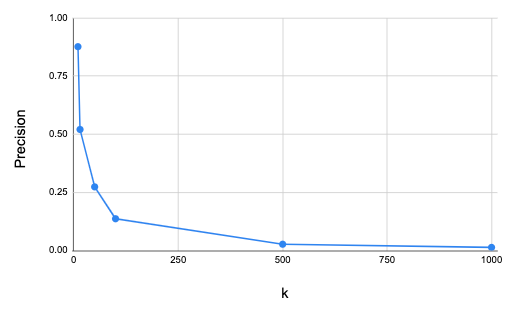
\includegraphics[width=0.48\linewidth]{spark-precision-k.png} & 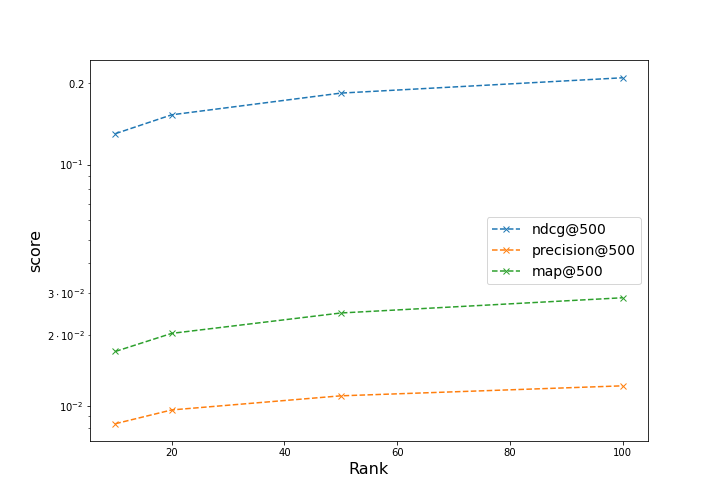
\includegraphics[width=0.48\linewidth]{lenskit-rank.png}
    \end{tabular}
    \caption{
    (\textbf{Left}) With the \texttt{precision@k} metric, we find that performance drops with increasing $k$. This may be attributed to the fact that most users have few ($\ll$ 500) relevant items.
    (\textbf{Right}) Performance improves overall as rank increases.
    }
    \label{fig:precision_k_and_rank}
\end{figure}

\paragraph{Model Tuning} We implemented three models: a baseline model with Spark ALS, a single-machine implementation of ALS using LensKit, and a popularity-based Bias model using LensKit. 

For both of the ALS models, we performed grid search over the following parameters where the values in bold were found to be the best configuration. In addition, we tried a broader range of values but did not find a significant difference. We found running ALS for a maximum of $20$ iterations was enough to reach convergence.

\begin{itemize}
\item $Rank$: [10, 20, 50, \textbf{100}] - size of the latent factors.
\item $\lambda$: [0.1, \textbf{1}, 10] - regularization parameter that controls the model complexity to prevent overfitting.
\item $\alpha$: [\textbf{10}, 20, 40] - scale factor to compute the each user-item weighting $c_{ui}$, as in \cref{eq:rec_obj_implicit}.
\end{itemize}

We found that rank has a significant positive correlation with model performance across all three metrics (\cref{fig:precision_k_and_rank}), whereas the other parameters had negligible impact. This is likely due to the large size of training data and the model requiring more latent factors to learn from patterns within the training set. Additionally, the model is more likely to underfit rather than overfit given a large dataset, so the influnece of the regularization parameter weakens. There is, however, a performance-time tradeoff, as higher rank results in longer time to fit.

For the popularity-based model, we investigated the impact of providing the model with either implicit or explicit feedback. We implemented a count-to-rating conversion function as described in \cref{sec:extensions}, ran the model with $\beta_u=100$ and $\beta_i=330$ on subsampled data of various sizes, then compared performance of the model when provided with count-based and rating-based data.
As the following two tables illustrate, we found the outcome to be similar bewteen the two, and decided to continue experimentation with count-based data.

\begin{table}[h]
    \begin{minipage}{.5\textwidth}
        \centering
        \begin{tabular}{cccc}
        \hline 
        \textbf{Size} & \textbf{Precision} & \textbf{MAP} & \textbf{NDCG}\\ 
        \hline
        14 k & 0.0228 & 0.0057 & 0.0484  \\
        91 k & 0.0139 & 0.0054 & 0.0431  \\
        570 k & 0.1224 & 0.2781 & 0.4871  \\
        3.21 M & 0.1246 & 0.6620 & 0.8039  \\
        \hline
        \end{tabular}
        \caption{Original Count Performance for Popularity-based model}
    \end{minipage}
    \hfill
    \begin{minipage}{.5\textwidth}
        \centering
        \begin{tabular}{cccc}
        \hline 
        \textbf{Size} & \textbf{Precision} & \textbf{MAP} & \textbf{NDCG} \\ 
        \hline
        14 k & 0.0228 & 0.0058 & 0.0486  \\
        91 k & 0.0139 & 0.0063 & 0.0460  \\
        570 k & 0.1224 & 0.2945 & 0.4961  \\
        3.21 M & 0.1246 & 0.6736 & 0.8084  \\
        \hline
        \end{tabular}
        \caption{Rating Transfer Performance for Popularity-based model}
    \end{minipage}
\end{table}

\paragraph{Model Comparison} We evaluated the test set against all three models with their best configurations. \cref{table:2} details the scores per each evaluation metric as well as total computation time taken for training and evaluation on the full dataset.

\begin{table}[H]
\centering
\begin{tabular}{c c c c c}
\hline 
\textbf{Model} & \textbf{Precision@500} & \textbf{MAP} & \textbf{NDCG@500} & \textbf{Computation Time(s)} \\ 
\hline
Popularity-based & 0.0243 & 0.84244 & 0.9031 & 308.95 \\
LensKit ALS (CG) & 0.0121 & 0.0286 & 0.209 & 33039.15 \\
Spark ALS & \textbf{0.0274} & 1.0000 & 1.0000 & \textbf{175.1451} \\
\hline
\end{tabular}
\caption{Comparing the three models, we find that Spark ALS provides the best speed and performance in terms of all metrics. The computation time represents the total time taken for model training and evaluation. The unusually high values for \texttt{MAP} and \texttt{ndcg@500} may  be  caused  by  bugs in the evaluation logic. The performance of LensKit ALS may have suffered due to unconverged conjugate gradients.}
\label{table:2}
\end{table}

When comparing the two ALS model implementations, we can observe that the Spark version ran about 189 times faster than the single-machine implementation in LensKit. For running the Spark ALS model on NYU Peel cluster, we configured for 12 cores and 16g memory.

Note that MAP and NDCG scores appear suspiciously high for both the Spark ALS model and the Popularity-based LensKit model; we believe these may be caused by bugs in the evaluation logic, which was implemented from scratch.

\newpage
\section*{Contributions}

\textbf{Zheyuan Hu} - LensKit Recommendation Model \& Experimentation, Writing. \\
\textbf{Ye Eun Jeong} - Data Preprocessing, Spark ALS Model Tuning \& Experimentation, Writing. \\
\textbf{Sanyam Kapoor} - Data Subsampling, Ranking Metric Queries, ALS Model Tuning \& Experimentation, Writing. \\
\textbf{Hongmiao Yu} - Popularity Bias Model \& Experimentation, Writing.

\bibliography{references}

\clearpage
\appendix

\section{Dropping low count entries}

As noted earlier, we also investigate the effect of dropping the interactions with counts lower than a threshold $N$. We observe that it does not improve the performance in terms of \texttt{precision@500}. The behavior is demonstrated by \cref{fig:precision_drop_count}.

\begin{figure}[!ht]
    \centering
    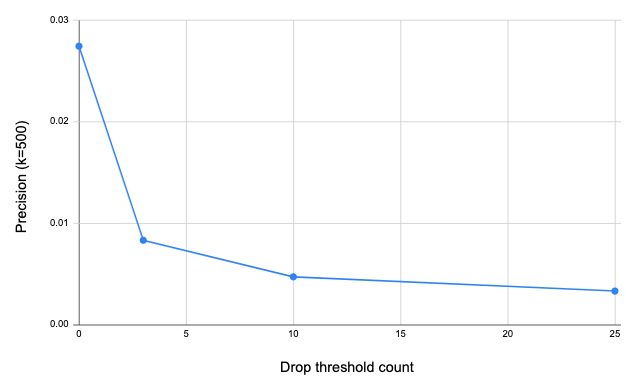
\includegraphics[width=0.5\linewidth]{spark-als-precision-dropcount.png}
    \caption{Dropping rows with low counts leads to loss in performance, understandably due to loss of information from the \emph{zero} interactions.}
    \label{fig:precision_drop_count}
\end{figure}



\section{Ranking Metrics}
\begin{table}[H]
\centering
\begin{tabular}{|>{\centering\arraybackslash}m{2.2cm}|>{\centering\arraybackslash} m{6cm}|>{\arraybackslash} m{5.8cm}|}
\hline 
\textbf{Metric} & \textbf{Mathematical Definition} & \textbf{Description} \\ 
\hline

Precision at k (k=500)
& $\frac{1}{M} \sum_{i=0}^{M-1} {\frac{1}{k} \sum_{j=0}^{\text{min}(Q_i, k) - 1} rel_{D_i}(R_i(j))}$  
& {A measure of how many of the first k recommended documents are in the set of true relevant documents averaged across all users.} \\
\hline
MAP
& $\frac{1}{M} \sum_{i=0}^{M-1} {\frac{1}{N_i} \sum_{j=0}^{Q_i-1} \frac{rel_{D_i}(R_i(j))}{j + 1}}$
& {A measure of how many of the recommended documents are in the set of true relevant documents}\\
\hline
NDCG at k (k=500)
& $\frac{1}{M} \sum_{i=0}^{M-1} {\frac{1}{IDCG(D_i, k)}\sum_{j=0}^{n-1} \frac{rel_{D_i}(R_i(j))}{\text{log}(j+2)}} $
& {A measure of how many of the first k recommended documents are in the set of true relevant documents averaged across all users.} \\
        
\hline
\end{tabular}
\caption{Ranking Metrics}
\label{4}
\end{table}

\end{document}